

%%%%%%%%%%

\begin{frame}{\Large \vskip -0.1cm R.A. Fisher's Iris Dataset\;\;\small(3 species, 50 records each)
\vskip -0.2cm{\tiny Fisher, R.A. \textit{The use of multiple measurements in taxonomic problems}, Annual Eugenics, 7, Part II, 179-188 (1936)}
}

\small

\begin{multicols}{2}

	\begin{flushleft}
	%\mbox{} \vskip -0.75cm
	\begin{minipage}{4.5cm}
	\vskip -0.2cm
	\begin{center}
	$\textnormal{Iris setosa}$
	\vskip 0.05cm
	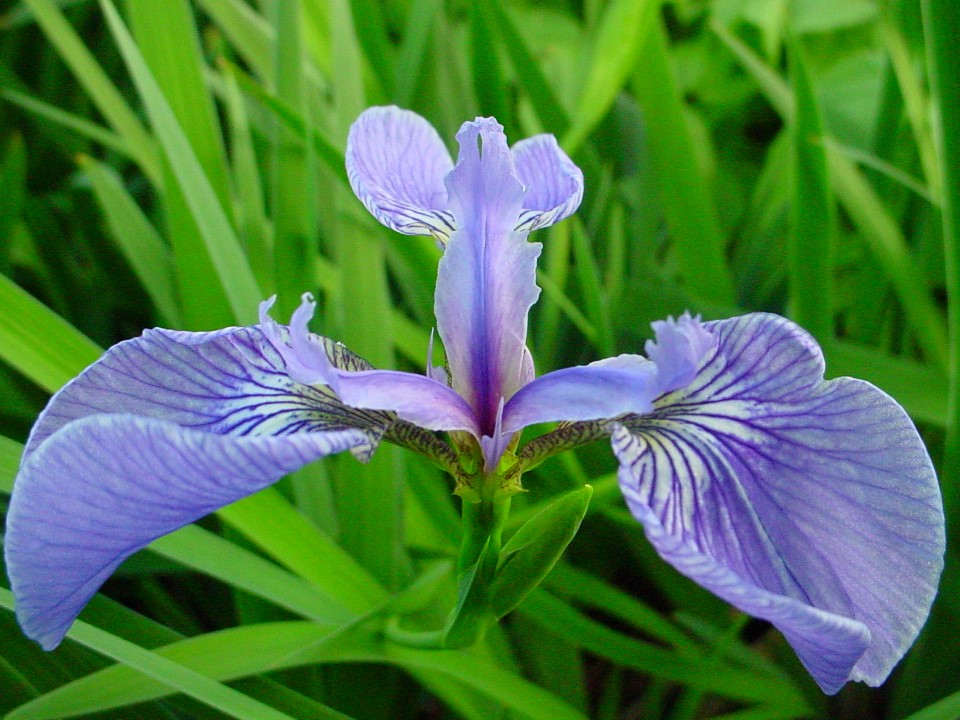
\includegraphics[width=3.5cm]{graphics/Iris-setosa-var-canadensis.png}
	\end{center}
	\end{minipage}
	\end{flushleft}

\columnbreak

	\begin{flushright}
	\begin{minipage}{4.5cm}
	\vskip -0.2cm
	\begin{center}
	$\textnormal{Iris versicolor}$
	\vskip 0.05cm
	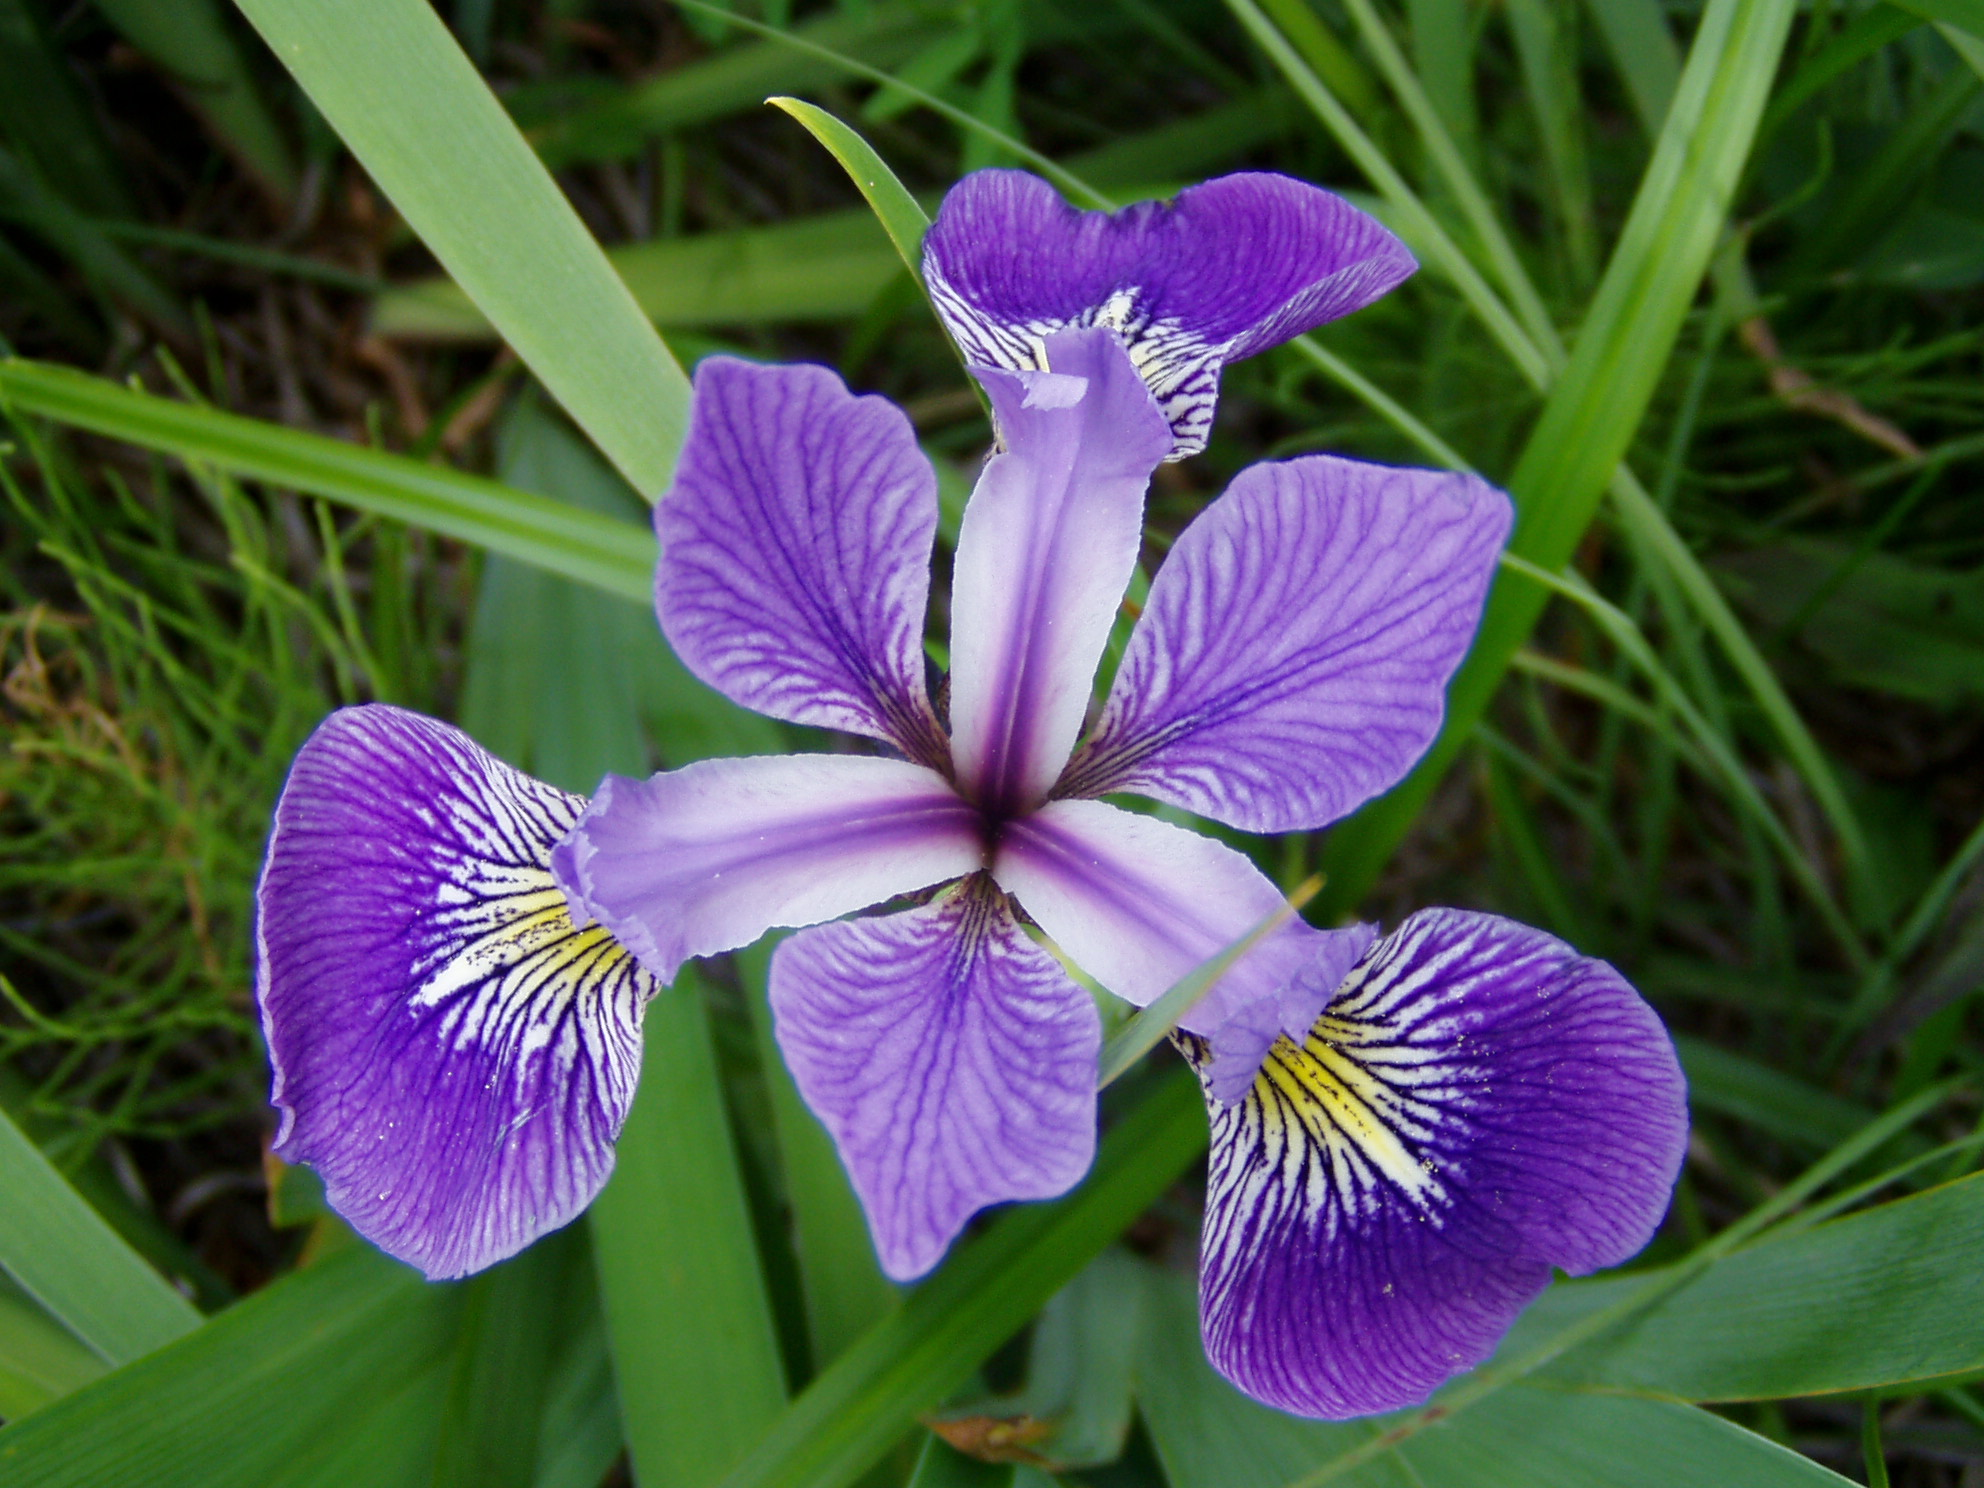
\includegraphics[width=3.5cm]{graphics/Iris-versicolor-3.png}
	\end{center}
	\end{minipage}
	\end{flushright}

\end{multicols}

\begin{multicols}{2}

	\begin{flushleft}
	\begin{minipage}{4.5cm}
	%\vskip -0.2cm
	\begin{center}
	$\textnormal{Iris virginica}$
	\vskip 0.05cm
	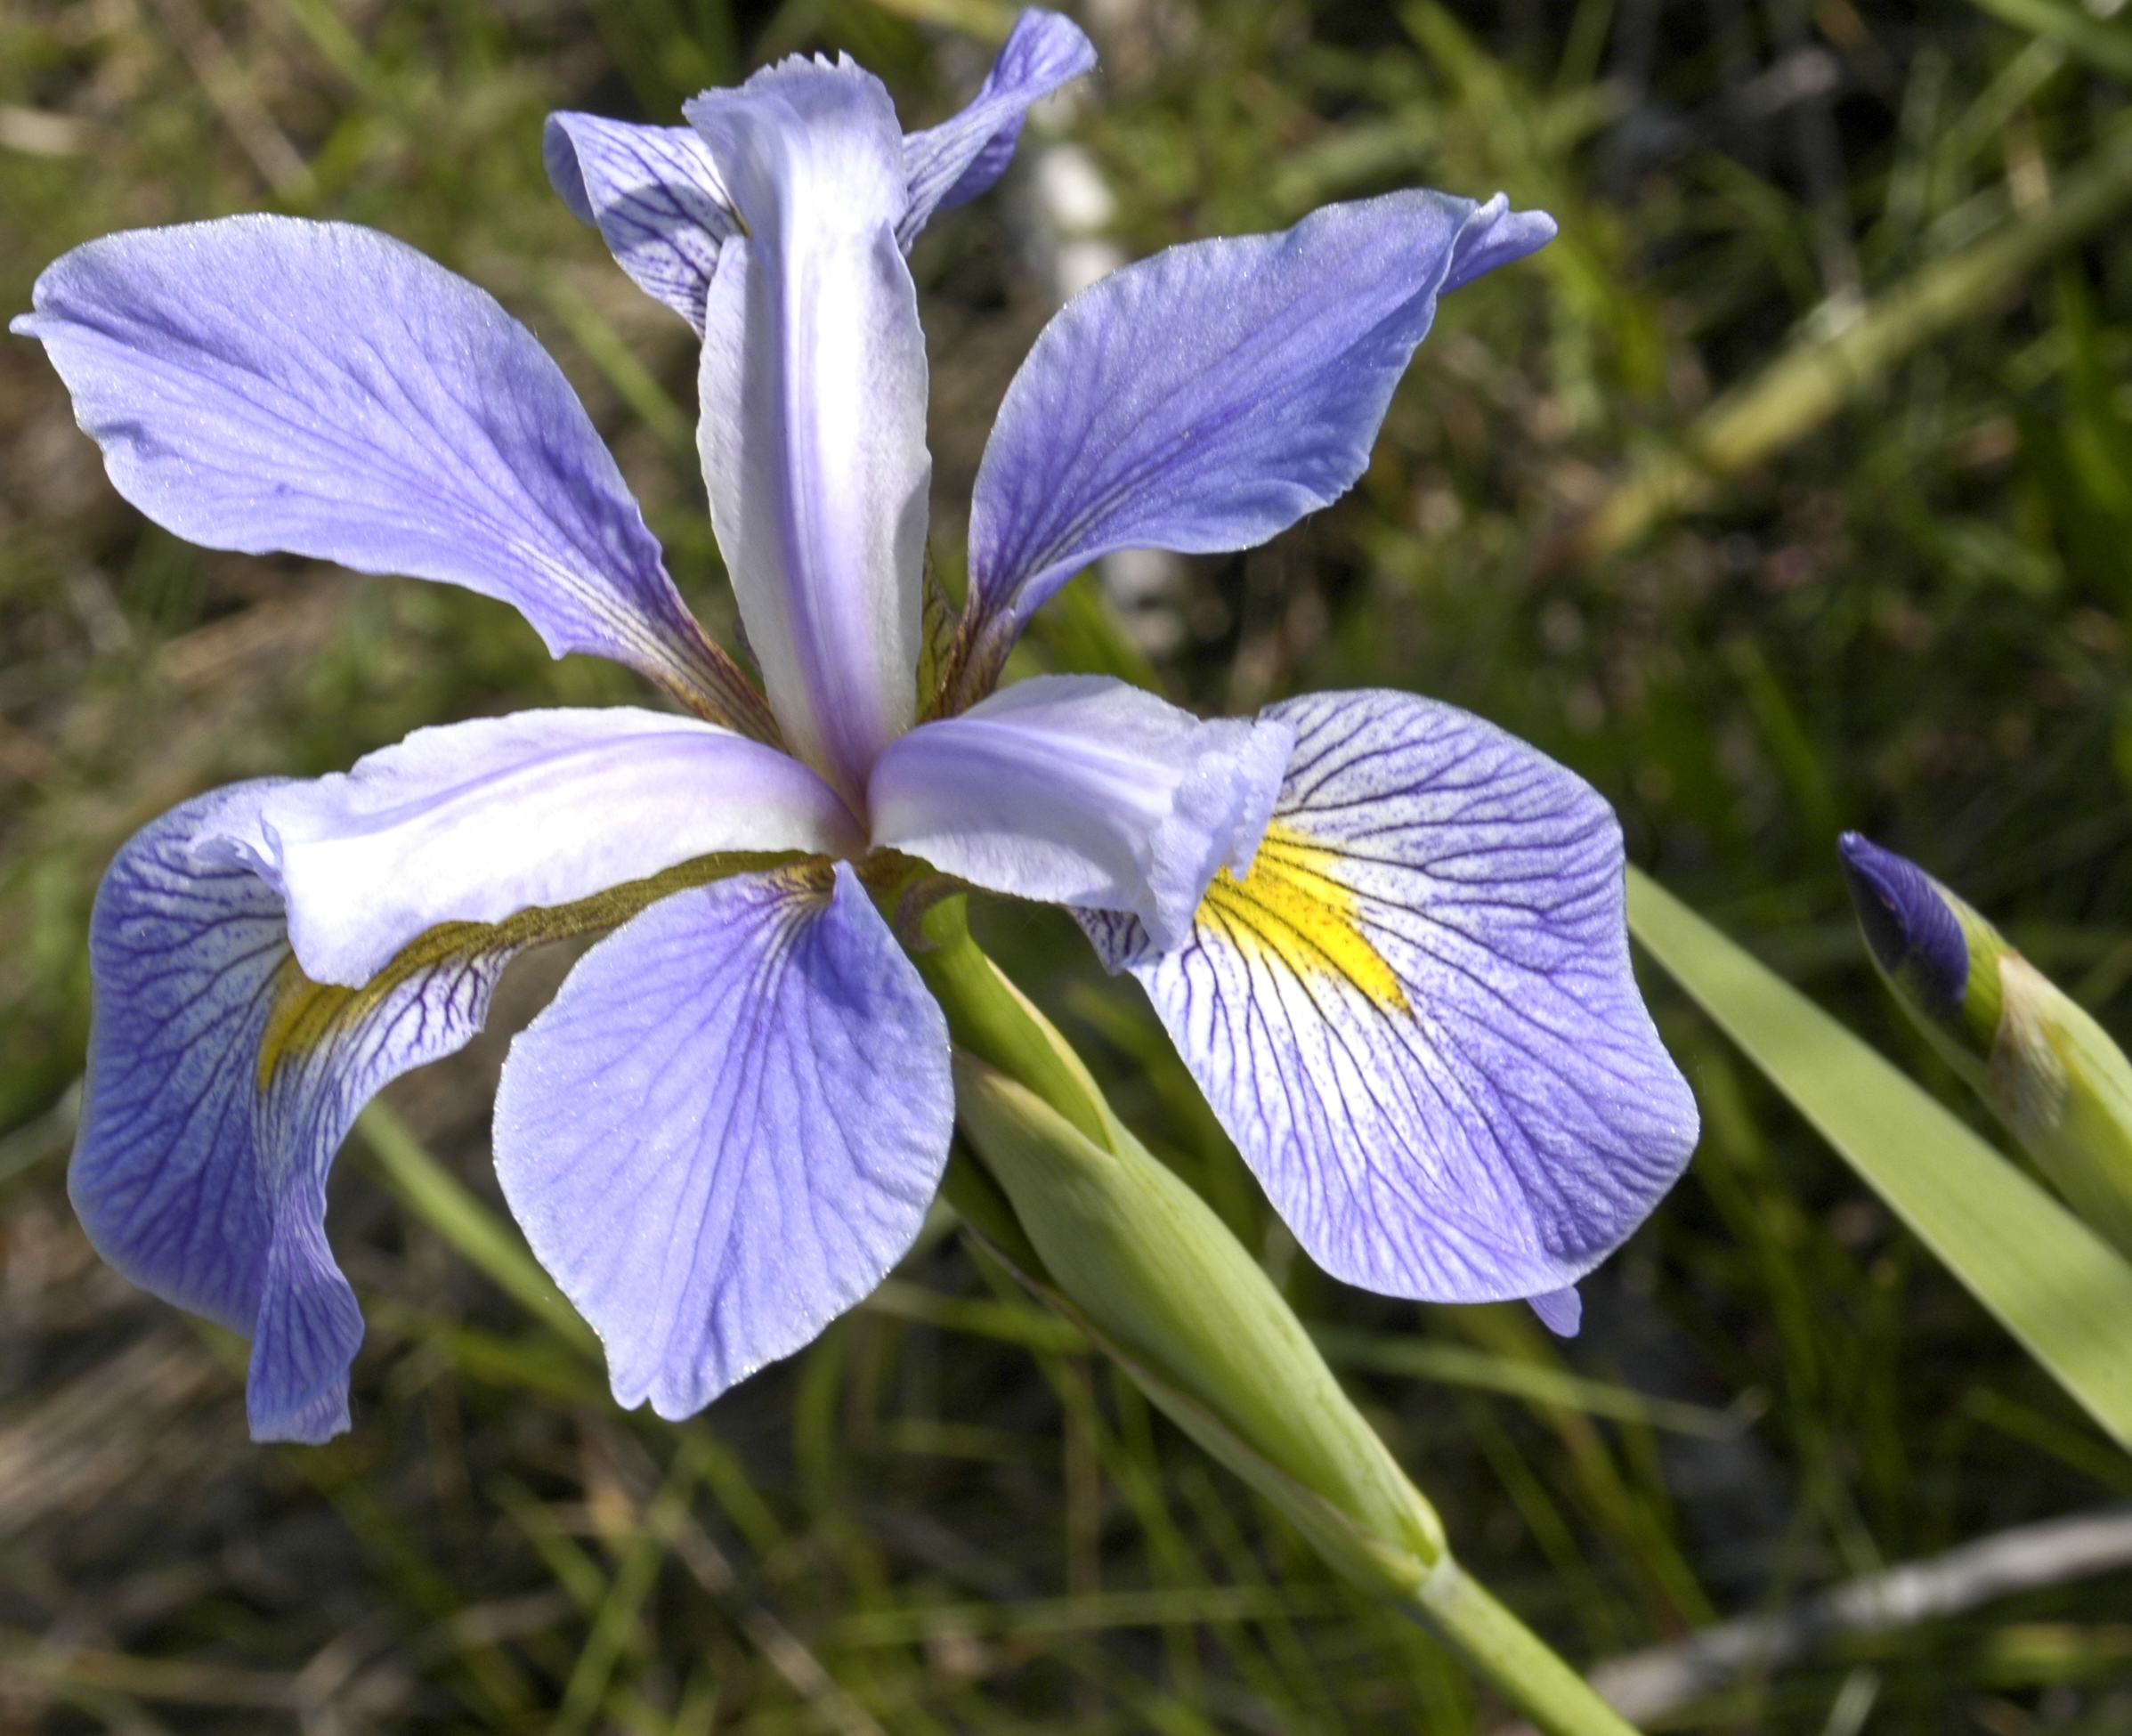
\includegraphics[width=3.5cm]{graphics/Iris-virginica.png}
	\end{center}
	\end{minipage}
	\end{flushleft}

\columnbreak

	\begin{flushright}
	\begin{minipage}{4.5cm}
	%\vskip -0.2cm
	\begin{center}
	\includegraphics[width=3.0cm]{graphics/iris-petal-sepal-278x300.png}
	\end{center}
	\end{minipage}
	\end{flushright}

\end{multicols}

\end{frame}
\normalsize

%%%%%%%%%%

\begin{frame}{\large Fitting a classification tree with R's \texttt{rpart(\,)}}

\small

\begin{multicols}{2}

	\begin{flushleft}
	\begin{minipage}{4.5cm}
	\only<1-2|handout:0>{\includegraphics[width=4.5cm]{graphics/scatter-petalLength-vs-petalWidth.png}}
	\only<3-3>{\includegraphics[width=4.5cm]{graphics/scatter-petalLength-vs-petalWidth-boundaries.png}}
	\end{minipage}
	\end{flushleft}

\columnbreak

	\begin{flushright}
	\begin{minipage}{4.5cm}
	\vskip -0.55cm
	\only<1-1|handout:0>{\includegraphics[width=4.5cm,height=6.75cm]{graphics/transparent.png}}
	\only<2-3>{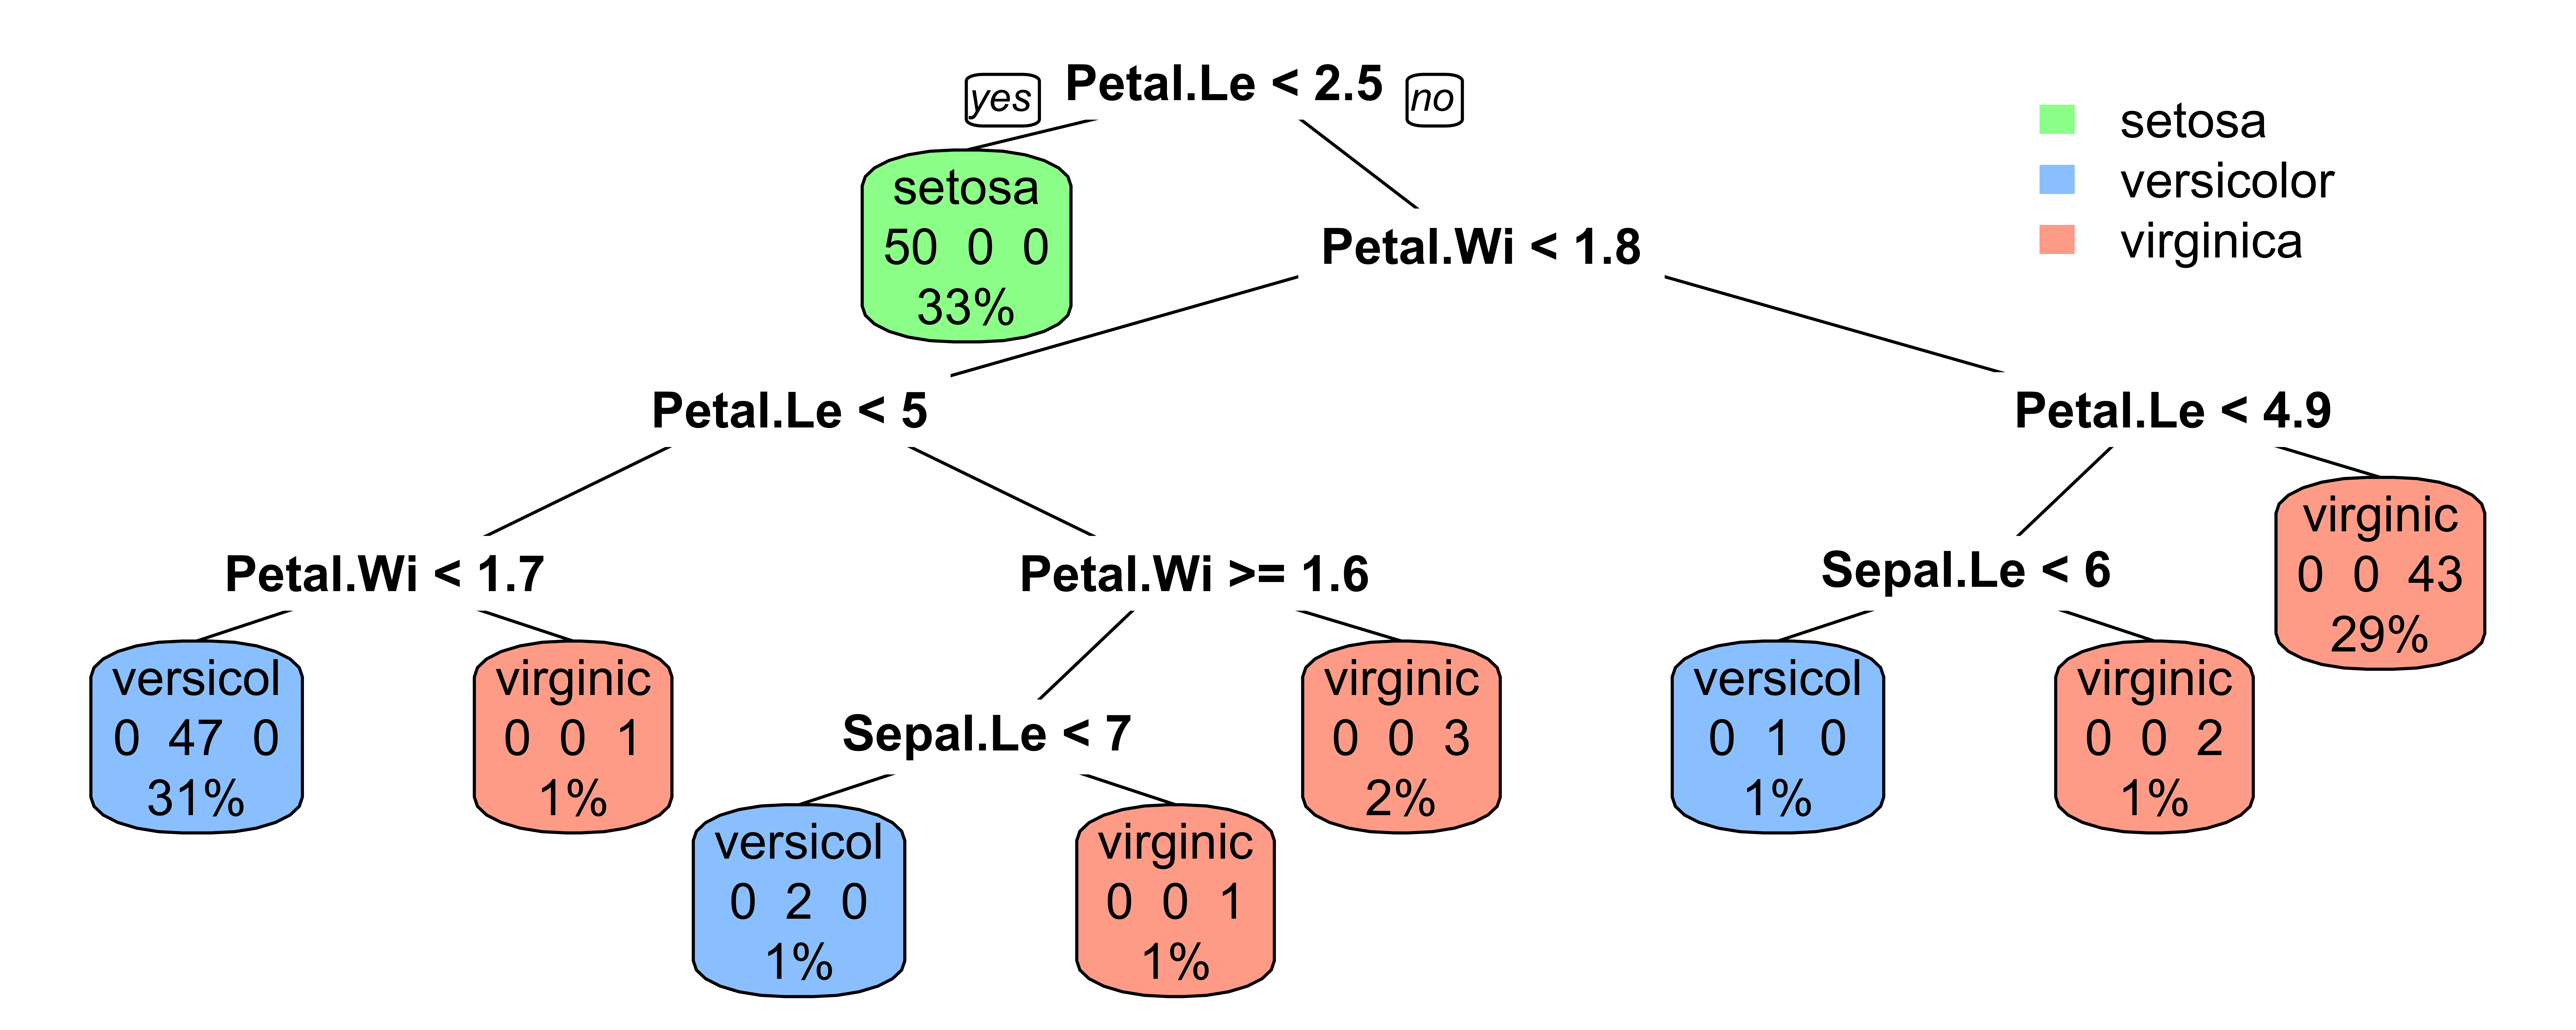
\includegraphics[width=4.5cm,height=6.75cm]{graphics/plot-rpart.png}}
	\end{minipage}
	\end{flushright}

\end{multicols}

\end{frame}
\normalsize

%%%%%%%%%%

\begin{frame}{\vskip -0.4cm \small Piecewise constant functions generated by\\ \textbf{\Large recursive binary partitioning}}

\small

\begin{multicols}{2}

	\begin{flushleft}
	\begin{minipage}{4.5cm}
	\includegraphics[width=4.5cm]{graphics/scatter-petalLength-vs-petalWidth-boundaries.png}
	\end{minipage}
	\end{flushleft}

\columnbreak

	\begin{flushleft}
	\begin{minipage}{4.5cm}
	\vskip -0.55cm
	\includegraphics[width=5.5cm,height=6.75cm]{graphics/plot-regression-surface.png}
	\end{minipage}
	\end{flushleft}

\end{multicols}

\end{frame}
\normalsize

%%%%%%%%%%
